\documentclass[preview]{standalone}

\usepackage{amsmath}
\usepackage{amssymb}
\usepackage{tikz}
\usepackage{graphicx}
\usepackage{pgfplots}
\usepackage{amsmath}
\usepackage{stellar}

\hypersetup{
    colorlinks=true,
    linkcolor=black,
    urlcolor=blue,
    pdftitle={Vectors},
    pdfpagemode=FullScreen,
}

\begin{document}

\title{Vectors}
\id{vectors}
\genpage

\section{Definition}

\includesnpt{linearalgebra-vector-definition}

\section{Addition}

\begin{snippet}{vector-addition}
Vectors can be added together. This operation is commutative.

\[
    \vec{a} + \vec{b} = \vec{c}
\]\phantom{}
\end{snippet}

\subsection{Graphically}

\begin{snippet}{vector-addition-geometric}
This plot shows how two vectors are added together in a two-dimensional space.

\begin{center}
	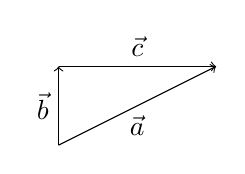
\begin{tikzpicture}
		\draw [->] (1,1) -- node [below] {\(\vec{a}\)} (3,2);
		\draw [->] (1,1) -- node [left] {\(\vec{b}\)} (1,2);
		\draw [->] (1,2) -- node [above] {\(\vec{c}\)} (3,2);
	\end{tikzpicture}
\end{center}
\end{snippet}

\subsection{Using its components}

\begin{snippet}{vector-addition-components}
The respective components of the vectors can be added to perform vector addition.

\[
    \vec{a} + \vec{b} =
    \begin{pmatrix}
        \vec{a}_1 \\
        \vec{a}_2 \\
        \vdots \\
        \vec{a}_n
    \end{pmatrix}
    +
    \begin{pmatrix}
        \vec{b}_1 \\
        \vec{b}_2 \\
        \vdots \\
        \vec{b}_n
    \end{pmatrix}
    =
    \begin{pmatrix}
        \vec{a}_1 + \vec{b}_1 \\
        \vec{a}_2 + \vec{b}_2\\
        \vdots \\
        \vec{a}_n + \vec{b}_n
    \end{pmatrix}
\]
\phantom{}
\end{snippet}

\section{Scalar Product}

\begin{snippet}{scalar-product}
A vector \(\vec{a}\) can be multiplied by a scalar value \(k\)

\[
    k\cdot\vec{a} =
    \begin{pmatrix}
        k \vec{a}_1 \\
        k \vec{a}_2 \\
        \vdots \\
        k \vec{a}_n
    \end{pmatrix},
    \quad k\in\mathbb{R}
\]\phantom{}
\end{snippet}

\section{Linear Combination}

\subsection{Definition}

\includesnpt{linearalgebra-linear-combination-definition}

\subsection{Span}

\includesnpt{linearalgebra-span-definition}

\subsection{Linear dependency}

\begin{snippet}{vector-linearly-independent}
Whenever you can remove a vector from a set of vectors without reducing the span,
the vectors are \textit{linearly dependent}.
One of the vectors of this set can be expressed as a linear combination of the other vectors in the span.

%Two vectors are collinear if one is a scalar multiple of the other 

%\[
%    \vec{v}_1 = a\cdot\vec{v}_2
%\]

If every vector in the set extends the span, they are \textit{linearly independent}.
\end{snippet}

\section{Magnitude}

\begin{snippet}{vector-magnitude}
To find the magnitude (or length) of a vector \(\vec{a}\) we can apply Pythagorean theorem.

\[
    ||\vec{a}|| = \sqrt{{a_x}^2 + {a_y}^2}
\]

For an n-dimensional vector.

\[
    ||\vec{a}|| = \sqrt{{a_1}^2 + {a_1}^2 + \cdots + {a_n}^2},
    \quad \vec{a}\in\mathbb{R}^n
\]\phantom{}
\end{snippet}

\section{Vector given points}

\begin{snippet}{vector-given-points}
We can find a vector given two points \(A\) and \(B\).

\begin{align*}
    &A(A_x; A_y) \\
    &B(B_x; B_y)
\end{align*}

The vector with direction going from \(A\) to \(B\) is given by

\[
    \begin{pmatrix}
        B_x - A_x \\
        B_y - A_y
    \end{pmatrix}
\]

For \({{\mathbb{R}}^n}\)

\[
    \begin{pmatrix}
        B_1 - A_1 \\
        B_2 - A_2 \\
        \vdots \\
        B_n - A_n
    \end{pmatrix}
\]\phantom{}
\end{snippet}

\section{Unitary Vector}

\begin{snippet}{unitary-vector-definition}
A unitary vector (or normalized vector) is a vector of magnitude \(1\).

\[
    ||\hat{a}|| = 1
\]

To normalize a vector it is sufficient to divide its components by its magnitude

\[
    \frac{\vec{a}}{||\vec{a}||}=\hat{a}
\]

\(\vec{a}\) can't be the \textit{null} vector.
\end{snippet}

\section{Basis}

\begin{snippet}{basis-definition}
A set of vectors in a vector space is called a \textit{basis} if every element
of the vector space can be expressed as a linear combination of the \textit{basis vectors}.

This means that the span of a basis is always every possible vector.

\[
    \mathcal{B} =
    \left\{
        \vec{b_1}, 
        \vec{b_2}, 
        \cdots,
        \vec{b_n}
    \right\},
    \quad \forall\, \vec{b} \in \mathcal{B}, \vec{b} \in {\mathbb{R}}^n
\]

In other words a \textit{basis} of a vector space is a set of
linearly independent vectors that span the full vector space.
\end{snippet}

\subsection{Orthonormal basis}

\begin{snippet}{orthonormal-basis}
An Orthonormal basis in a basis in which each vector is orthogonal to eachother and every vector
is unitary.

% generalize example

Given a basis \(\{\vec{i}, \vec{j}\}\)

\[
    \vec{v} = a \cdot \hat{i} + b \cdot \hat{j},
    \quad a,b \in \mathbb{R}
\]

\begin{enumerate} % i don't like this
    \item \(\hat{i}\) is perpendicular to \(\hat{j}\)
    \item \(\hat{i}\) and \(\hat{j}\) are unitary
    \item \(\hat{i} \neq a\cdot\hat{j},\quad a\in \mathbb{R}\)  
\end{enumerate}
\end{snippet}

\end{document}
